\chapter{Component Based Architecture}
\label{chp_cba}
In this chapter we introduce the notion of \textit{Component Based Architecture} (CBA), in order to give context to the data set and problem we aim to solve with machine learning. First of all, we briefly cover the motivation for developing CBA application. Then, we proceed to the definition of a software component and how they are connected to create a functional software application. Finally, we introduce system logs and the structure of these.


\section{Overview and Software Design}
CBA has turned into an appealing software design paradigm for software oriented corporations, such as Ericsson. This is due to two things; firstly, it is a way for a company to shorten the development time for their software applications. Secondly, CBA makes it easier to manage the software as components are designed with reusability and replacement in mind \cite{ericssonCBA}.  


\subsection{Components}
A software component is a modular software object that encapsulates some predefined functionality in the overall set functionality provided by the entire CBA application. To better understand a software component we use the definition of the three properties that defines a component according to Szyperski et al. \cite{Szyperski:2002:CSB:515228}. First, a component has to be \textit{independently deployable}, which means that its inner functionality is shielded from the outer environment. The property also excludes the ability for a component to be deployed partially. Secondly, a component has to be a \textit{self-contained entity in a configuration of components}. In order for a component to be self-contained, a specification of requirements has to be clearly stated, together with the services it provides. This is achieved by having well-defined interfaces. An interface acts as an access point to the inner functionality, where the components are able to send and receive instructions or data. A component usually have multiple interfaces, where different interfaces allows clients, i.e. other components or systems, to invoke different services provided. However, to properly function, components also have to specify their dependencies, which define rules for the deployment, installation, and activation of the specific component. We illustrate the first two properties with an abstract CBA application in \autoref{fig:cba_fig}. Finally, a component can not have \textit{externally observable states}, which means that internal states can be cached or erased, without major consequences to the overall application. 


\begin{figure}[H]
    \centering
    \scalebox{.5}{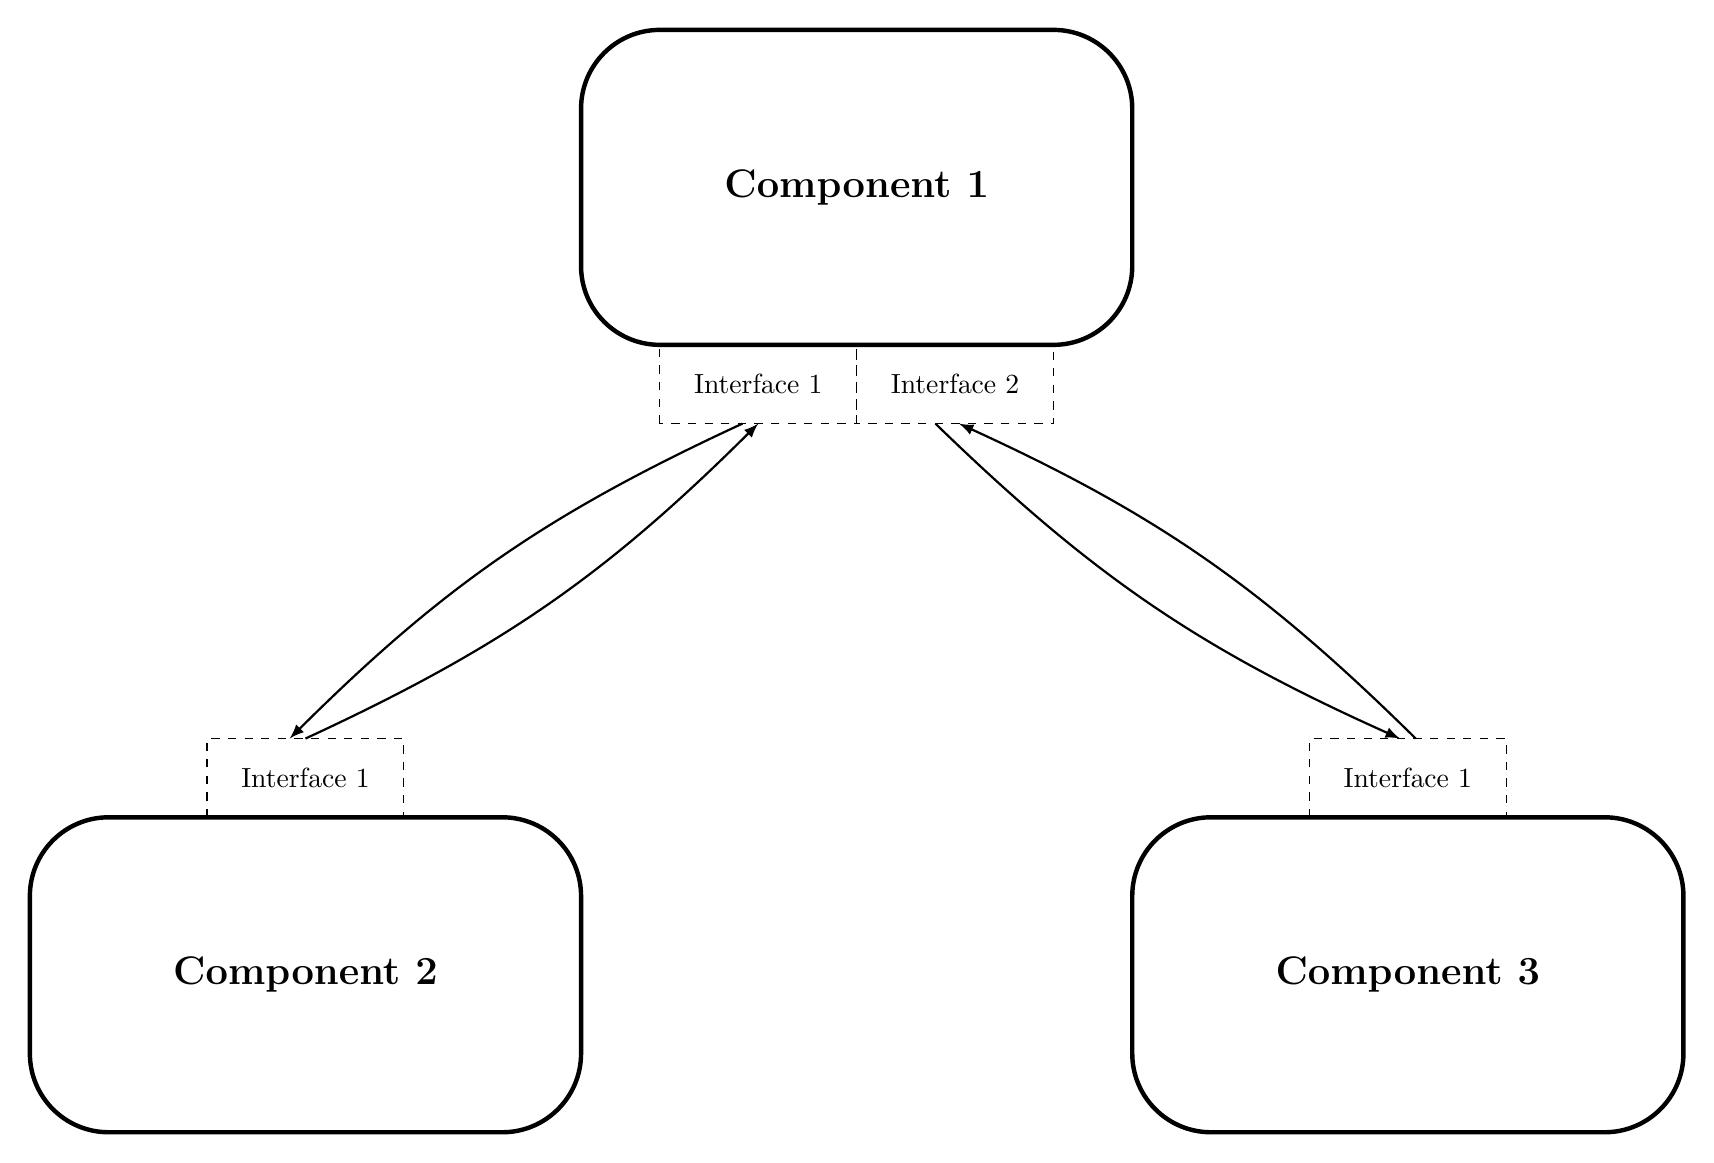
\begin{tikzpicture}


\draw [rounded corners=1cm,ultra thick] (0,0) rectangle ++(7,4) node [midway] {\Large\textbf{Component 1}};

\draw [dashed] (1,-1) rectangle ++(2.5,1) node [midway] {Interface 1};

\draw [dashed] (3.5,-1) rectangle ++(2.5,1) node [midway] {Interface 2};

\draw [rounded corners=1cm,ultra thick] (-7,-10) rectangle ++(7,4) node [midway] {\Large\textbf{Component 2}};

\draw [dashed] (-4.75,-6) rectangle ++(2.5,1) node [midway] {Interface 1};

\draw[-latex,thick] (-3.5,-5) to[bend right=10] (2.25,-1);

\draw[-latex,thick] (2.05,-1) to[bend right=10] (-3.7,-5);

%\draw[latex'-latex',ultra thick](-4,-5) to (2.25,-1);

\draw [rounded corners=1cm,ultra thick] (7,-10) rectangle ++(7,4) node [midway] {\Large\textbf{Component 3}};

\draw [dashed] (9.25,-6) rectangle ++(2.5,1) node [midway] {Interface 1};

\draw[-latex,thick] (10.6,-5) to[bend right=10] (4.8,-1);

\draw[-latex,thick] (4.5,-1) to[bend right=10] (10.4,-5);


\end{tikzpicture}}
    \caption{An abstract illustration of a CBA application of three components interacting via their interfaces.}
    \label{fig:cba_fig}
\end{figure}


\subsection{Challenges in Development of CBA Applications}
A CBA application consist of a topology of interconnected components, as shown in \autoref{fig:cba_fig}, where each component is responsible for some part of the overall system functionality. Individual components are built using traditional software engineering principles, which means that they are developed and tested in isolation before full-scale system integration and testing. Thus, errors usually occur due to the composition of the CBA application, where unforeseen states of component can cause them to fail \cite{Szyperski:2002:CSB:515228}. To find out which components failed during system integration, a technician usually has to go through the system logs generated during the testing in order to find the cause of failure. As this is a time consuming work for a technician, the aim is to automate this task. To get a better understanding of the challenges when trying to automate this task we now proceed to go through the structure of the system logs generated in the test suite environment. 

\section{System Logs}
System logs are generated in test suites, where all events executed are recorded in system log files. The structure of system logs we analyse in this thesis is presented in \autoref{fig:syslog_struct}.


\begin{figure}[H]
    \centering
        \begin{verbatim}
         
        Time_stamp Log_location process[PID]: Description
    
        \end{verbatim}
    \caption{The general structure of a system log.}
    \label{fig:syslog_struct}
\end{figure}

\noindent To understand each term of the system log we will go through them one by one.

\begin{itemize}[leftmargin=4em,align=left]
    
    \item \verb|Time_stamp| -- At which time the event was executed/logged.
    
    \item \verb|Log_location| -- The system log will either be logged in a \textit{system controller} or in a \textit{system Payload}, denoted \textit{SC} and \textit{PL} respectively.
    
    \item \verb|process| -- The name of the process that executed the command.
    
    \item \verb|[PID]:| -- The process identification, surrounded by brackets and ending with a colon.
    
    \item \verb|Description| -- States what occurred or action taken, and in some cases the severity level of the event.

\end{itemize}

\noindent The first three terms of the system log are rather self explanatory and thus we will not go into them any further. However, description is the term that is most important to solving the task of making the analysis of system logs autonomous. The description include information such as, severity, e.g. \textit{error} or \textit{rebooting}, effected components and their states, and sometimes a reason is stated. The challenge with the description is however that they do not follow a set of predefined rules, and are generally ill-structured. The reason for this is that each system log is written by a specific software engineering team who developed that component. Each software team or developer has their own unique style and selection of acronyms that becomes troublesome. Due to format and inconsistency of the description, it will impact the ability of the machine learning models to learn the patterns that separate the individual fault classes in the system logs. We have now introduced the general structure of the data set and we will now proceed to the theory of the machine learning model we will use.


To summarise this chapter; we started off by introducing the reason for component based software applications. Then, we briefly defined what a software component is and how it interacts with its environment. Next, we proceeded to state the challenges in the development of CBA systems. Finally, the general structure of the system logs was stated to get a context to the data set and its limitations.